% ============================================================
% Bangun Datar untuk Soal Geometri - pendamping artikel blog
% https://pakgun.gezytech.web.id/tikz-bangun-datar-soal-geometri/
% Kompilasi: pdflatex (butuh paket tikz)
% ============================================================
\documentclass{article}
\usepackage[a4paper, margin=2cm]{geometry}
\usepackage{amsmath}
\usepackage{tikz}

\begin{document}

\section*{1. Segitiga siku-siku untuk soal Pythagoras}

Satu unit TikZ = satu sentimeter, koordinat langsung terbaca:

\begin{tikzpicture}[scale=0.8]
  \draw[thick] (0,0) -- (6,0) -- (6,8) -- cycle;
  \draw[thick] (5.7,0) -- (5.7,0.3) -- (6,0.3); % siku di C
  \draw (3,0) node[below] {$6$ cm};
  \draw (6,4) node[right] {$8$ cm};
  \draw (0,0) node[below left] {$A$};
  \draw (6,0) node[below right] {$B$};
  \draw (6,8) node[above right] {$C$};
\end{tikzpicture}

\section*{2. Trapesium sama kaki (sisi sejajar 10 cm dan 6 cm, tinggi 4 cm)}

Selisih sisi sejajar $=4$ cm, dibagi dua $=2$ cm — titik miring mundur 2 cm:

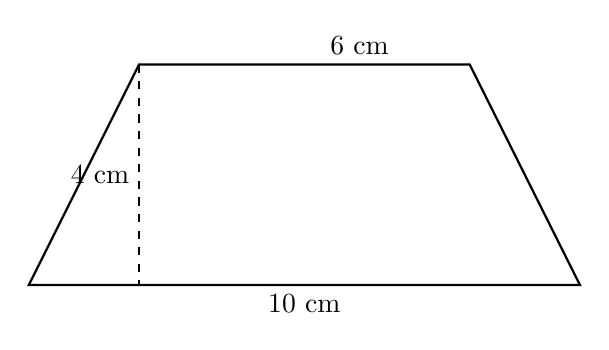
\begin{tikzpicture}[scale=0.7]
  \draw[thick] (0,0) -- (10,0) -- (8,4) -- (2,4) -- cycle;
  \draw[dashed] (2,4) -- (2,0);
  \draw (6,4) node[above] {$6\ \text{cm}$};
  \draw (5,0) node[below] {$10\ \text{cm}$};
  \draw (2,2) node[left] {$4\ \text{cm}$};
\end{tikzpicture}

\section*{3. Lingkaran dengan jari-jari yang tembus ke tepi}

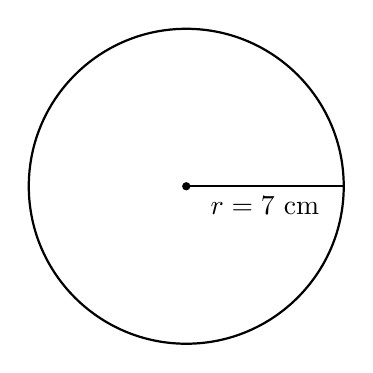
\begin{tikzpicture}
  \draw[thick] (0,0) circle (2);
  \draw[thick] (0,0) -- (2,0) node[midway, below] {$r = 7$ cm};
  \fill (0,0) circle (1.5pt);
\end{tikzpicture}

\end{document}
